%&latex
\documentclass[letterpaper]{article}
\usepackage{aaai}
\usepackage{amsfonts}
\usepackage{times}
\usepackage{helvet}
\usepackage{courier}
\usepackage{ifthen}
\usepackage{color}

\nocopyright

\newcommand{\fix}[1]{{$\langle${\sc #1}$\rangle$}}
\newcommand{\comment}[1]{{\color{blue}{#1}}}

\usepackage[pdftex]{graphicx}
\usepackage{amsmath}

\newcounter{codeline}
\newenvironment{code}{
  \newcommand{\cl}{ % code line
    \refstepcounter{codeline}
    \ifthenelse{\value{codeline}<10}{\hspace{5pt}\arabic{codeline}}{\arabic{codeline}}.
  }
  \begin{tabbing}
    00. nn\=nn\=nn\=nn\=nn\=nn\=nn\=nn\=nn\=nn\kill
} {\end{tabbing}}

% italics in math mode
\newcommand{\myit}[1]{\mbox{\em #1}}
% in subscripts
\newcommand{\myits}[1]{\mbox{\scriptsize \em #1}}

\newcommand{\citep}[1]{\citeauthor{#1}~\shortcite{#1}}
\newcommand{\citeq}[1]{\citeauthor{#1}~\citeyear{#1}}

\newcommand{\fromM}[1]{{$\langle${\sc M: #1}$\rangle$}}
\newcommand{\pv}{\myit{PlanVisioner }}

% evil
%\def\baselinestretch{.968}
%\setlength\textheight{9.12in}
%\setlength\textwidth{7.1in}
%\setlength\columnsep{0.245in}

\def\europa{{\sl EUROPA}}

\newcommand{\figwidth}[2]{\mbox{\resizebox{#1}{!}
{\includegraphics{#2}}}}

\newcommand{\fixE}[1]{$\langle${\sc EB: #1}$\rangle$}

%------------------------------
\begin{document}

\title{\europa: A Platform for AI Planning, Scheduling, Constraint Programming, and Optimization}


\author{Javier Barreiro, Matthew Boyce, Jeremy Frank, Michael Iatauro, Tatiana Kichkaylo, Paul Morris, Tristan Smith, Minh Do}

%Keywords: Planning, real-time}


\date{}
\maketitle

%------
\begin{abstract}

\europa is a class library and tool set for building and analyzing planners (and/or schedulers) within a Constraint-based Temporal Planning paradigm. This paradigm has been successfully applied in a wide range of practical planning problems and has a legacy of success in NASA applications. \europa\ offers capabilities in 3 key areas of problem solving: (1) Representation; (2) Reasoning; and (3) Search. \europa\ is a means to integrate advanced planning, scheduling and constraint reasoning into an end-user application and is designed to be open and extendable to accommodate diverse and highly specialized problem solving techniques within a common design framework and around a common technology core.  In this paper, we will demonstrate the core capabilities of this open-source planning \& scheduling framework. While \europa\ is the complete planning and scheduling software suite, we will concentrate on the aspects that are relevant to the knowledge engineering purpose: modeling language capabilities, model debugging and execution tools, and plan visualization and analysis.

\end{abstract}
%-----


%---------------------
\section{Introduction}
\label{sec:intro}

\europa\ (Extensible Universal Remote Operations Planning Architecture) is a class library and tool set for building planners (and/or schedulers) within a Constraint-based Temporal Planning paradigm ~\cite{frank:europa}. Constraint-based Temporal Planning (and Scheduling) is a paradigm of planning based on an explicit notion of time and a deep commitment to a constraint-based formulation of planning problems. This paradigm has been successfully applied in a wide range of practical planning problems and has a legacy of success in NASA applications including :

\begin{itemize}
\item Observation scheduling for the Hubble Telescope ~\cite{muscettola:1998}
\item Autonomous control of DS-1.
\item Ground-based activity planning for MER.
\item Autonomous control of EO-1.
\end{itemize}

\europa\ is now at version 2.6 and is the successor of the original \europa\ which in turn was based upon HSTS ~\cite{muscettola:1998}. It has been made available under an open-source license. The source code and extensive documents on \europa\ are available at: \emph{http://code.google.com/p/europa\-pso/}. As a Planning \& Scheduling Knowledge Engineering tool, \europa\ major strengths are: (1) flexibility in integrating with client applications; (2) proven track record; (3) open-source software license; (4) online document repository with detailed guidelines and a variety of examples in different domains.

\europa\ offers capabilities in 3 key areas of problem solving:

\begin{enumerate}
\item {\bf Representation}: \europa\ allows a rich representation for actions, states, resources and constraints that allows concise declarative descriptions of problem domains and powerful expressions of plan structure. This representation is supported with a high-level object-oriented modeling language for describing problem domains and data structures for instantiating and manipulating problem instances.
\item {\bf Reasoning}: Algorithms are provided which exploit the formal structure of problem representation to enforce domain rules and propagate consequences as updates are made to the problem state. These algorithms are based on logical inference and constraint-processing. Specialized techniques for reasoning about temporal quantities and relations included in \europa\ are particularly useful to deal with real-life problem domains.
\item {\bf Search}: Problem solving in \europa\ requires search. Effective problem solving typically requires heuristics to make search tractable and to find good solutions. \europa\ provides a framework for integrating heuristics into a basic search algorithm and for developing new search algorithms.
\end{enumerate}

\europa\ is not an end-user application. Rather, it is a means to integrate advanced planning, scheduling and constraint reasoning into an end-user application. \europa\ is not a specific planner or a scheduler. Rather it is a framework for developing specific planners and/or schedulers. It is designed to be open and extendable to accommodate diverse and highly specialized problem solving techniques within a common design framework and around a common technology core.

\europa\ is unconventional in providing a separate Plan Database that can integrate in a wide variety of applications. This reflects the common needs for representation and manipulation of plan data in different application contexts and different problem solving approaches. Possible approaches include:

\begin{itemize}
\item A batch planning application where an initial state is input and a final plan is output without any interaction with other actors.
\item A mixed-initiative planning application where human users interact directly with a plan database but also employ an automated problem solver to work on parts of the planning problem in an interleaved fashion.
\item An autonomous execution system where the plan database stores the plan data as it evolves in time, being updated from data in the environment, commitments from the executive, and the accompanying automated solver which plans ahead and fixes plans when they break.
\end{itemize}

While \europa\ is a large complex framework which provides many reasoning capabilities beyond the typical planning knowledge engineering tool, in this paper we will concentrate on aspects that are more relevant to IKEPS such as: modeling capabilities, model debugging and execution tools, and plan visualization and analysis. To emphasize the strength of \europa\ as a general purpose planning \& scheduling framework, we will include examples from different class of problems such as resource scheduling, simple planning domains (BlocksWorld), complex planning domains (Rovers), and CSP benchmarks (N-Queens)\footnote{All examples are included in the open-source distribution of \europa}. To give a more complete picture of the whole system, we will also provide a brief background on \europa\ main architecture and how key components are integrated.

For the rest of this paper, we will first outline the modeling and reasoning capabilities. We then provide a short guide on how to use \europa\ in the most effective way and illustrate it with a list of simple examples. We then list the NASA and non-NASA projects that have used \europa. We finish the paper with a brief discussion of related work and discussion of our product roadmap for future releases of \europa.


%-----------------------------
\section{Technical Background}

In this section, we will start with an introduction to \europa\ main modeling language with concentration on its modeling capabilities. We then follow with the brief description on \europa\ architecture and its key components. This will set the background for subsequent sections on knowledge engineering tools that are provided as part of the \europa\ distribution to assist with both the front-end (modeling assistant) and back-end (plan execution, visualization, and analysis) \comment{JRB: is this a standard definition of front-end back-end in KE?, doesn't strike me as intuitive}.

\subsection{\bf Modeling in NDDL}
\europa's main input modeling language is New Domain Definition Language (NDDL) (pronounced `noodle'), a domain description language for constraint-based planning and scheduling problems. NDDL can describe a number of concepts based on Variables and Constraints~\footnote{A complete NDDL Reference guide with examples is available at: \emph{http://code.google.com/p/europa-pso/wiki/NDDLReference} and the NDDL grammar guide is available at: \emph{http://code.google.com/p/europa-pso/source/browse/PLASMA/trunk/src/PLASMA/NDDL/ base/antlr/NDDL3.g}}. The NDDL representation includes state and activity descriptions, as is common in planners using traditional modeling languages like the Planning Domain Definition Language (PDDL) ~\cite{gerevini:ipcjair,hoffmann:ipcjair}.  However, unlike PDDL, NDDL uses a state variable-value formalism. \europa\ thus takes its heritage from planning formalisms like IxTeT ~\cite{ghallab:rci} and SAS ~\cite{jonsson:199}. \europa\ state variables are called timelines, and the values of timelines are sequences of states. States are temporally extended predicates, and consist of a proposition and a list of parameters, which by default includes the start, end and duration times.  Timelines are totally ordered sequences of states; hence, a timeline can be in only one state at any instant.  The final component of NDDL model is a set of compatibilities that govern the legal arrangements of states on, and across, timelines.  These compatibilities are logical implications asserting that if a timeline is in a state, then other timelines must be in one of a set of compatible states. Compatibilities can incorporate explicit constraints on the parameters of the states.  \europa\ provides a library of such constraints, and this library can be extended if new constraints are needed.
\comment{JRB: Timelines are a specific instance of the more general concept of Objects in europa, however, for this audience this description is probably appropriate}

There are several examples of NDDL for well known planning and CSP domains such as Blocksworld, 8-Queen, RCPSP available at the \europa\ website.
\comment{JRB: do we want to add a short nddl snippet that show the concepts mentioned above?}

\noindent {\bf  The NDDL Transaction Language:}
NDDL includes procedural extensions, referred to as the \emph{NDDL Transaction Language}, to operate on the plan database and thus initialize and/or modify a partial plan. A design goal of the NDDL transaction language is to provide syntax and semantics closely related to the use of NDDL elsewhere for class, predicate and rule declaration. However, the NDDL transaction language pertains exclusively to run-time data. It is referred to as a transaction language since a set of statements in this language form a procedurally executed sequence of atomic operations on the plan database, which stores an instance of a partial plan. Each statement of the language is thus directly translated into one or more operations available through the DbClient interface. The NDDL transaction language has many applications. The most common one is the construction of an initial partial plan as an input to a solver. A second important application is to log transactions on the plan database for later replay. This is useful for copying a database, and for reproducing a state found through planning in a direct manner without having to search. It is also a potentially very useful integration mechanism for pushing updates to the plan database from external systems.\\

\comment{JRB: do we want to add a short nddl snippet that show the concepts mentioned above?}


\noindent {\bf Supports for other Modeling Language:} At the current moment, we are adding support for ANML ~\cite{smith:anml}, the new modeling language that import features from PDDL, IxTeT, AML, and NDDL. Given that there are published works on the possible translation between ANML and PDDL
~\cite{smith:anml,smith:pddl-nddl}, we also plan to write the translator to support PDDL through ANML translation. 

%---------------------------
\subsection{\europa's Main Components}

Figure~\ref{fig:architecture} shows the main components of \europa\ and the relationships/interactions between them.
\comment{JRB: I replaced the figure with one that's more up to date, but we still need to include the UI and eclipse tools in it}

%--
\begin{figure}
  \begin{center}
    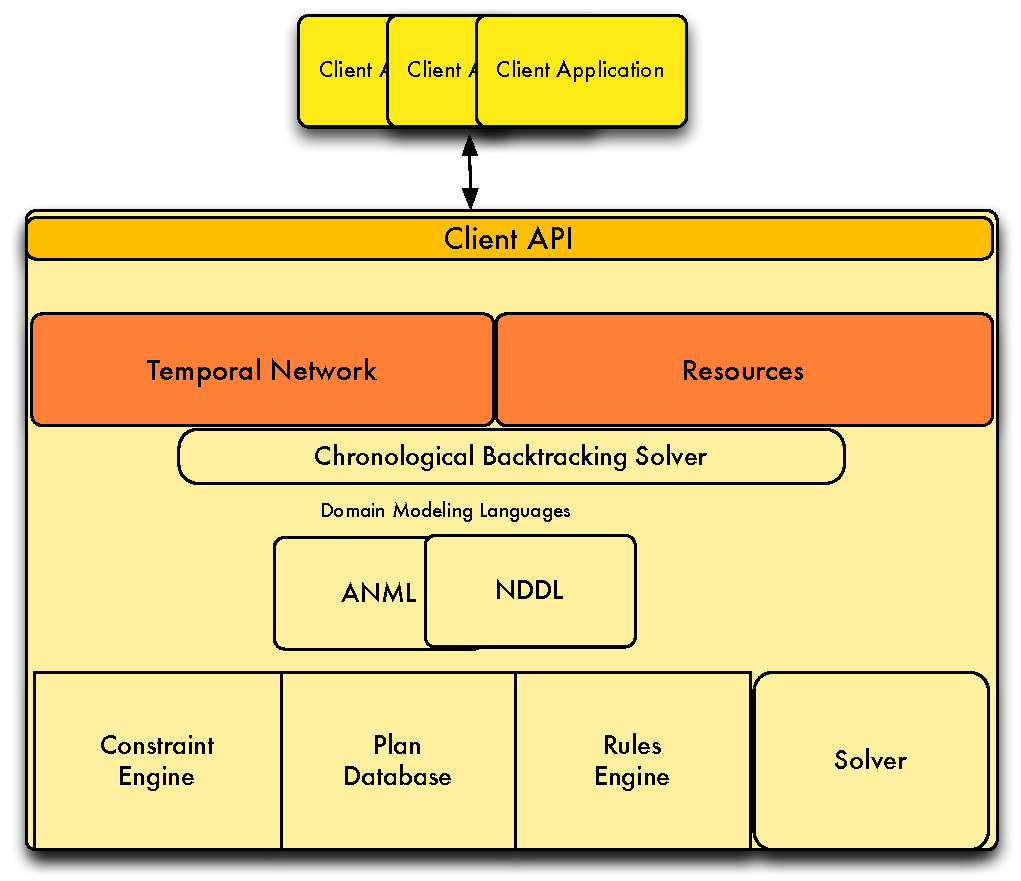
\includegraphics[width=3.5in]{./Figures/EUROPA-Architecture.pdf}
  \end{center}
%	\vspace*{-0.1in}
  \caption{\small \europa\ Architecture}
  \label{fig:architecture}
%  	\vspace*{-0.1in}
\end{figure}
%--

\comment{JRB: I'll have to update this section}

\noindent {\bf Utils module}: provides common C++ utility classes for error checking, smart pointers etc. It also includes a very useful debugging utility. Many common programming practices in \europa\ development are built on assets in this module.\\

\noindent {\bf Constraint Engine}: is the nexus for consistency management. It provides a general-purpose component-based architecture for handling dynamic constraint networks. It deals in variables and constraints. It includes an open propagation architecture making it straightforward to integrate specialized forms of local and global constraint propagation.\\

\noindent {\bf Plan Database}: adds higher levels of abstractions for tokens and objects and the interactions between them. This is the code embodiment of the \europa\ planning paradigm. It supports all services for creation, deletion, modification and inspection of partial plans. It maintains the dynamic constraint network underlying a partial�plan by delegation to the Constraint Engine and leverages that propagation infrastructure to maintain relationships between tokens and objects.\\

\noindent {\bf Solvers module}: provides abstractions to support search in line with the \europa\ planning approach. It includes a component-based architecture for Flaw Identification, Resolution and heuristics as well as an algorithm for chronological backtracking search. As additional search algorithms are implemented they will be added to this module.\\



%--
\begin{figure*}
  \begin{center}
    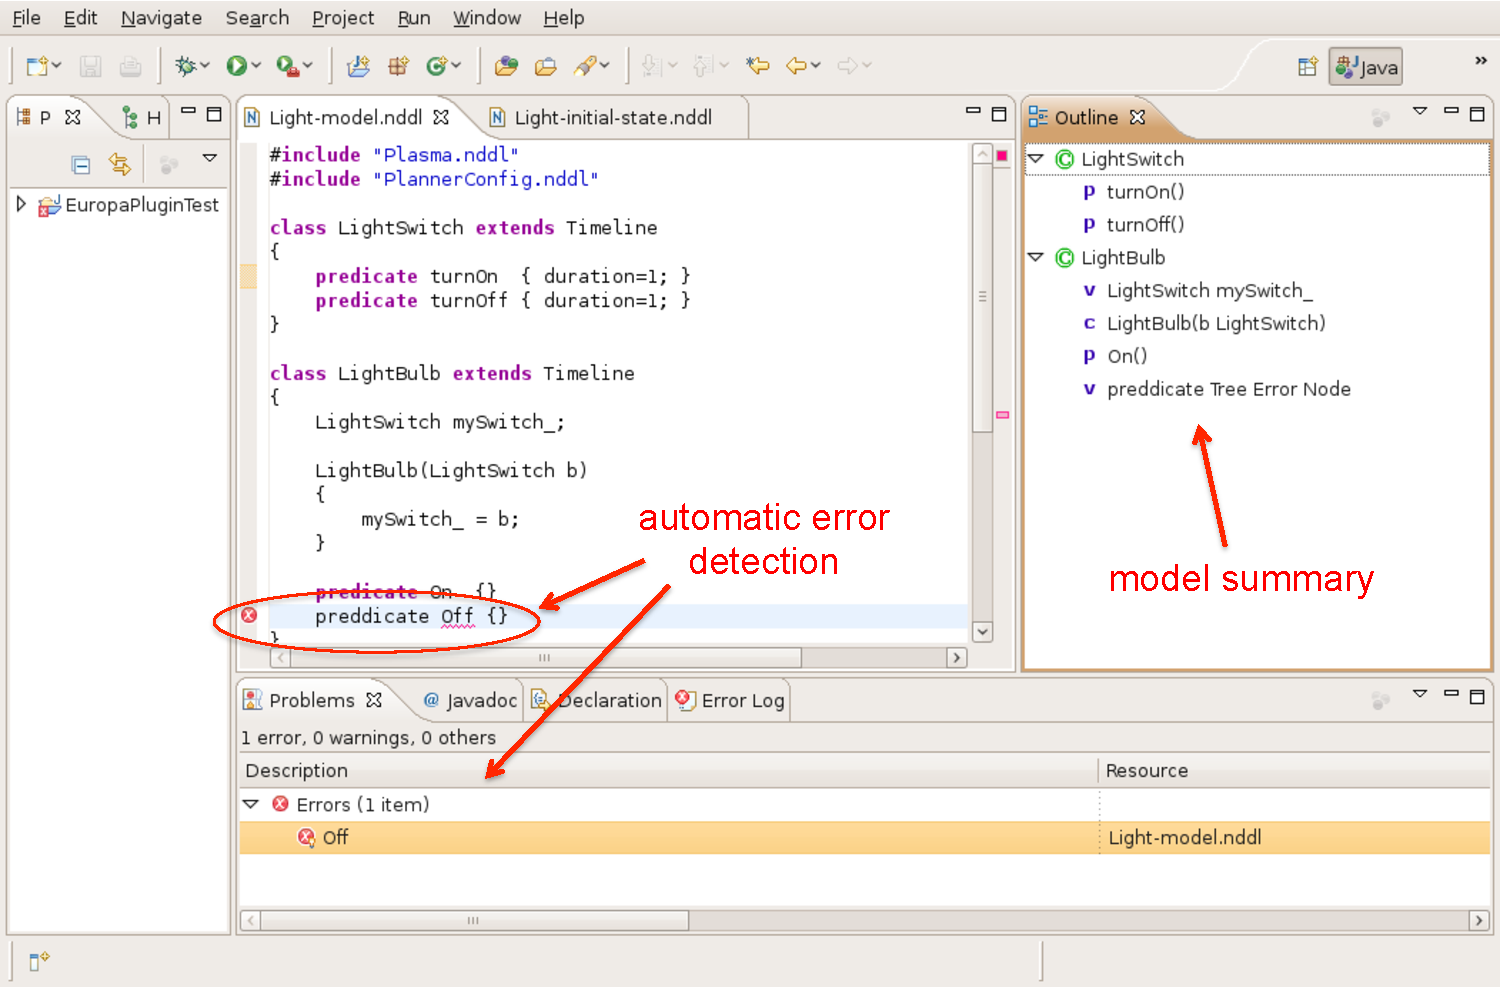
\includegraphics[width=6.5in]{./Figures/NDDL_editor.pdf}
  \end{center}
  \caption{\small NDDL Editor and Syntax Checker.}
  \label{fig:NDDL_editor}
\end{figure*}
%--


\noindent {\bf Rules Engine:} provides the inference capabilities based on domain rules described in the model. It is almost exclusively used to execute NDDL rules but can be extended for custom rule formats.\\

\noindent {\bf Resources module}:  provides specialized algorithms and data structures to support metric resources (e.g. battery, power bus, disk drive).
The Temporal Network module provides specialized algorithms and data structures to support efficient propagation of temporal constraints.\\

\noindent {\bf NDDL module}: provides a parser and compiler for NDDL (pronounced noodle) which is a very high-level, object-oriented, declarative domain and problem description language. This module defines the mapping from the language to the code and consequently interfaces to a number of key modules in the system.\\

From an application developer�s view-point, the modules of interest are: {\em NDDL}, {\em Solvers} and \comment{JRB: UI and eclipse tools?}. These modules address modeling, search and troubleshooting respectively. Other modules will be explored in the context of making customized extensions.



%---------------------------
\section{Using \europa\ \& its Supporting Tools}

There are several different ways in which \europa\ can be used to to support solving a planning \& scheduling or CSP problem: (1) embed \europa\ within the client application; (2) using \emph{PSDesktop}, a Java Swing UI Framework; and (3) using the provided Eclipse plugin. For the rest of this section, we will outline those three different approaches and provide some examples.


%------------------------------------
\subsection{Embed \europa\ in an Application}
\europa\ provides a script called \emph{makeproject} that will generate C++ and Java applications that embed \europa, along with simple NDDL model and initial-state files that users can then modify for their own purposes. This allows the users to perform the full application cycle of:

\begin{enumerate}
\item Initialize \europa\
\item Load/Modify model and initial state descriptions
\item Invoke a solver
\item Extract plan results from the Plan Database
\item Repeat steps 2-4 as many times as needed
\item Shutdown \europa\
\end{enumerate}

\comment{JRB: Provide a short snippet showing a  "hello world" java app that embeds europa?}

\noindent {\bf Using the C++ or JAVA API:} The \emph{PSEngine} interface is the official interface for \europa\ clients, it is the recommended way to use \europa. This interface is very straightforward and allows the user to run the entire application cycle described above. This abstraction layer will isolate a user's client code from most changes in the internals of the \europa\ implementation, it is also designed for easy mapping to other languages using SWIG.\\

\noindent {\bf Applications using different programming languages:} the corresponding binding for the \emph{PSEngine} interface should be either already available in the \europa\ distribution, or relatively easy to add. Note that while currently only Java bindings are bundled with the \europa\ distribution, we have plans to add Python and any other languages that are popular with the \europa\ user community~\footnote{This should not be too difficult given that SWIG supports many high-level programming languages.}.

%-----------
\subsection{JAVA Swing UI Framework}


%--
\begin{figure*}
  \begin{center}
    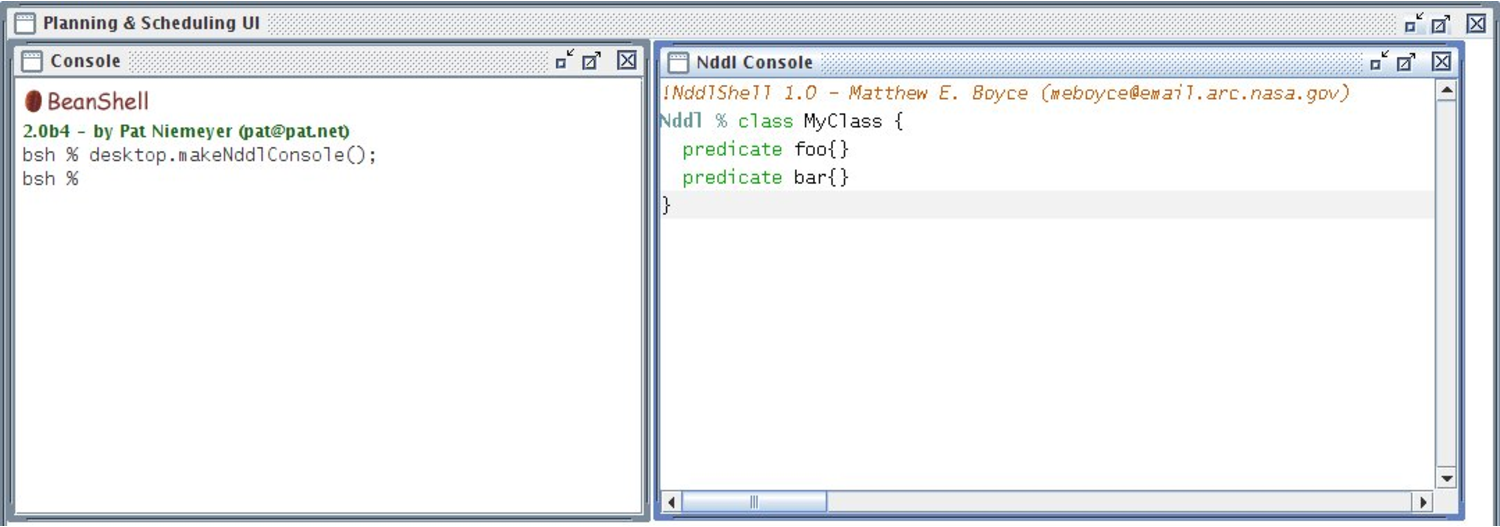
\includegraphics[width=6.5in]{./Figures/PSDesktop_1.pdf}
  \end{center}
  \caption{\small BeanShell and NDDL console windows}
  \label{fig:PSDesktop_start}
\end{figure*}
%--

%--
\begin{figure*}
  \begin{center}
    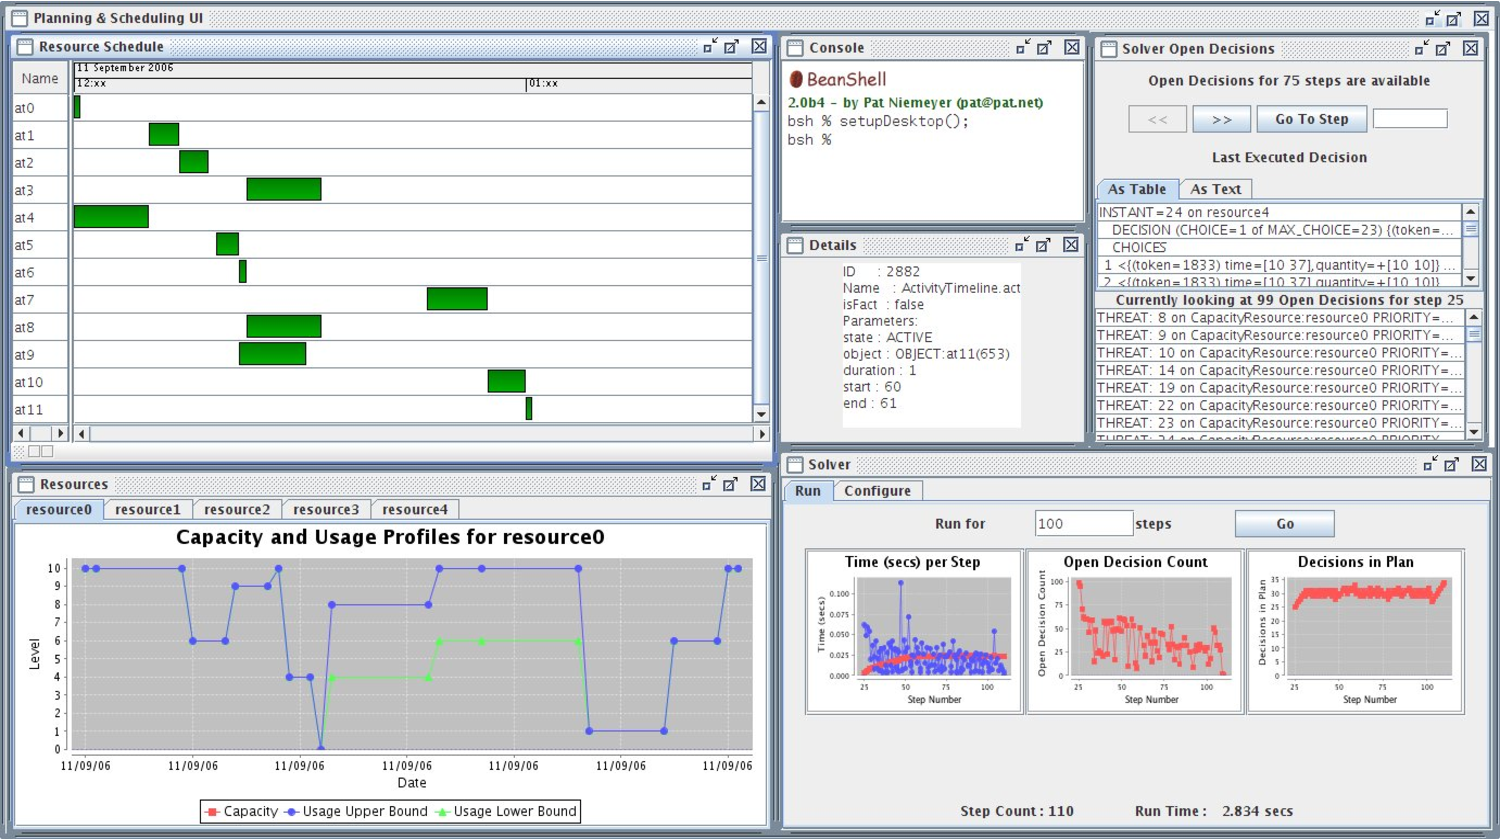
\includegraphics[width=6.5in]{./Figures/Example_UBO0.pdf}
  \end{center}
  \caption{\small Example of PSUI components}
  \label{fig:PSUI_exp}
\end{figure*}
%--



\emph{PSDesktop} is a Java application that allows the user to drive \europa\ interactively by making use of the \emph{PSEngine} client interface. It takes two arguments:

\begin{itemize}
\item To select \emph{Debug} or \emph{Optimized} version of \europa\ to run.
\item  \emph{bsh} file (optional) : filename of the \emph{BeanShell} file that is executed upon starting\footnote{BeanShell is a small, free, embeddable Java source interpreter with object scripting language features, written in Java. BeanShell dynamically executes standard Java syntax and extends it with common scripting conveniences such as loose types, commands, and method closures like those in Perl and JavaScript.}.
\end{itemize}

Figure~\ref{fig:PSDesktop_start} shows the two console windows when running {\em PSDesktop}. In the BeanShell console window you can type in Java statements that allow you to drive \europa\ interactively through its Java API. \comment{JRB: The NDDL console is currently broken!} In the NDDL console you can type in NDDL statements that will be interpreted as soon as you complete a valid NDDL statement and hit enter.\\

\noindent {\bf Interactive BeanShell Console:} In the BeanShell console, users will have access to the following variables :

\begin{itemize}
\item \emph{PSEngine}: this will give you access to the \europa\ engine, users can create a solver, query the plan database, execute NDDL scripts, in general perform any task needed to drive \europa\ to load a model and create a plan. Users can also use this interface to create your own custom solver.
\item \emph{PSDesktop}: this will give you access to many utility methods to create new desktop windows, display tables of tokens, create a solver, etc.
\end{itemize}


\noindent{\bf PSUI Components:} The PSUI package contains a number of components that make it easy to visualize your plan and interact with \europa\ :

\begin{itemize}
\item {\em PSGantt} : shows the tokens on a timeline as a gantt chart
\item {\em PSChart} : shows resource profiles as charts
\item {\em PSSolverDialog}: allows the user to drive a solver interactively and see its status as it tries to achieve the goals specified for it
\item {\em ActionDetails and ActionViolation}: enable easy display of violation and detail information about actions in a plan as the user mouses over actions in other components (for instance a gantt chart)
\end{itemize}

Figure~\ref{fig:PSUI_exp} shows an example of how different UI components within the PSUI package can be activated to assist the plan analysis.


%------------------
\subsection{Eclipse Plugin (SWT) for \europa\ Modeling, Solving, and Debugging}
The {\em Eclipse} plugin has two major components: (1) an editor and (2) an execution perspective. They provide the graphical interface to model, run, and analyze plans within the {\em Eclipse} development environment. The main capabilities are:

%--
\begin{figure*}
  \begin{center}
    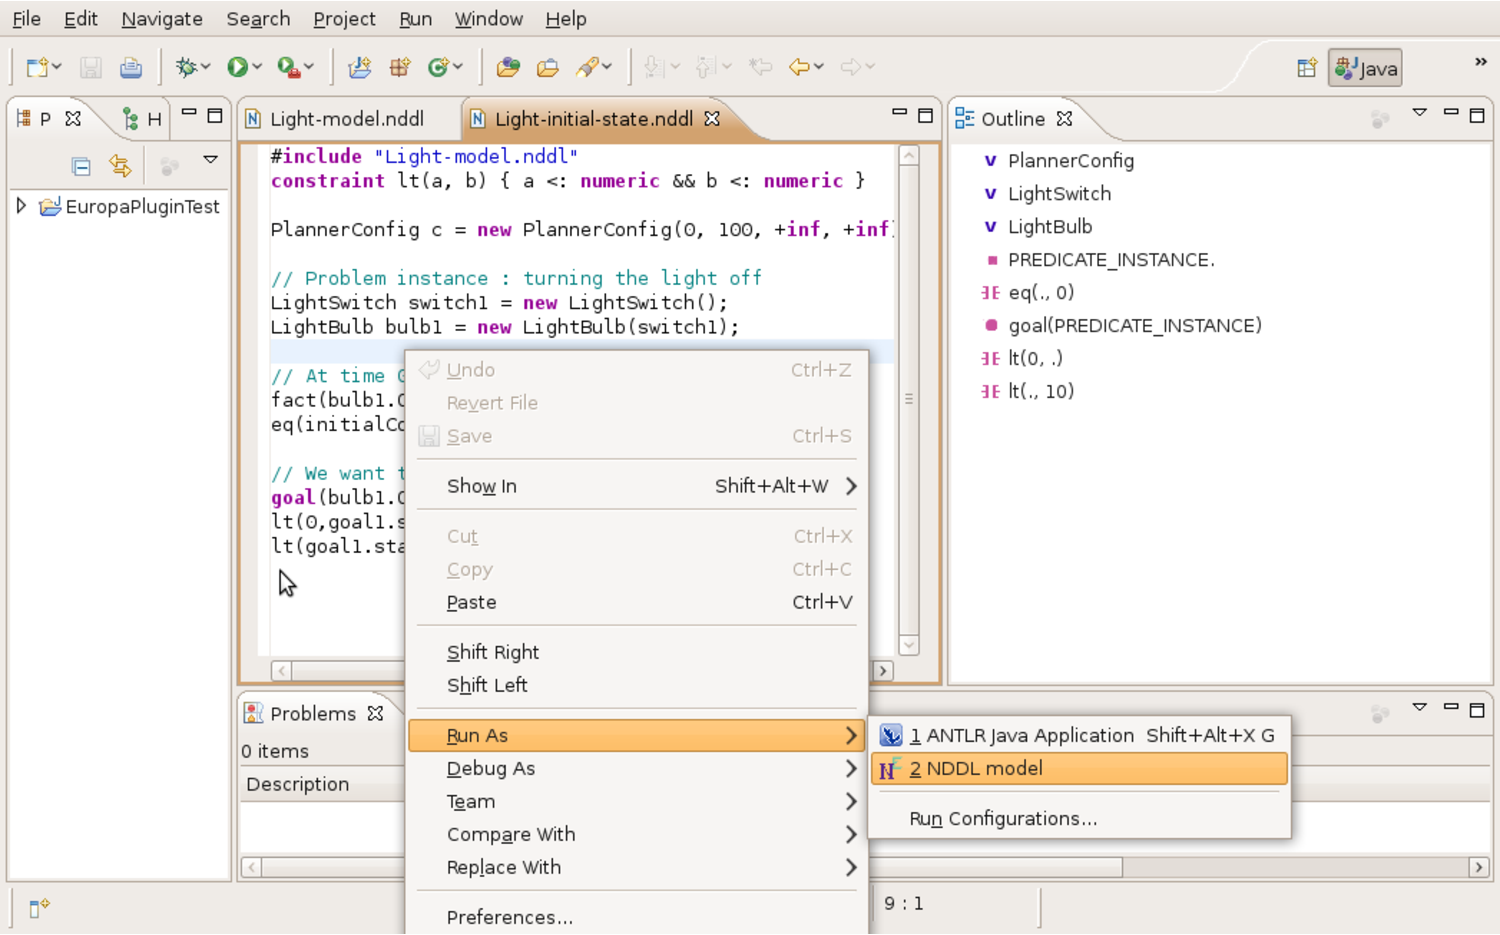
\includegraphics[width=6.5in]{./Figures/NDDL_runas.pdf}
  \end{center}
  \caption{\small Running a problem directly from the NDDL editor.}
  \label{fig:NDDL_runas}
\end{figure*}
%--

%--
\begin{figure*}
  \begin{center}
    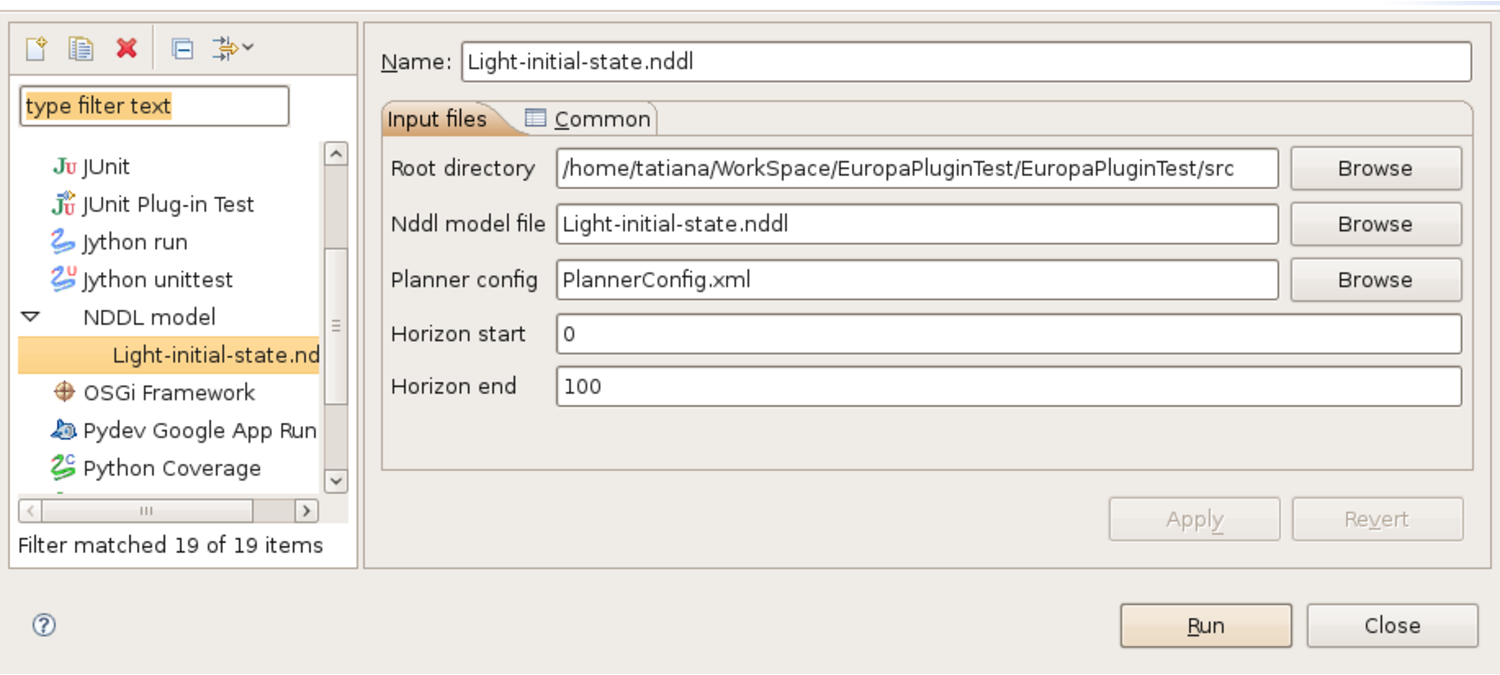
\includegraphics[width=6.5in]{./Figures/NDDL_runconfig.pdf}
  \end{center}
  \caption{\small Configurate a NDDL run.}
  \label{fig:NDDL_runconfig}
\end{figure*}
%--


%--
\begin{figure*}
  \begin{center}
    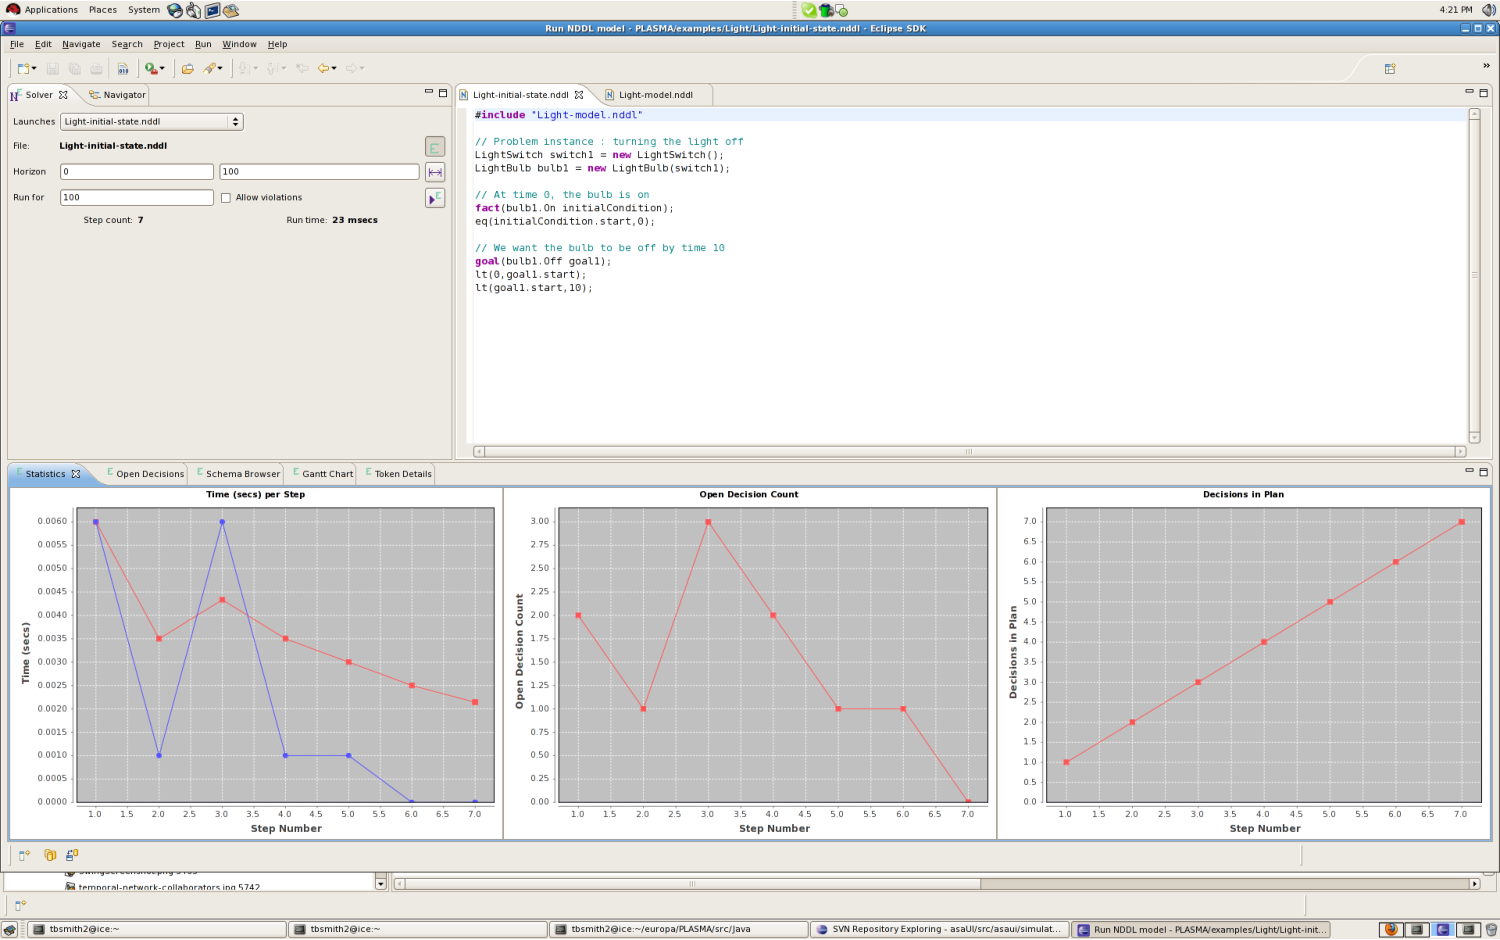
\includegraphics[width=6.5in]{./Figures/EclipseRunPerspective.pdf}
  \end{center}
  \caption{\small Eclipse dedicated perspective on showing information about running \europa}
  \label{fig:NDDL_runpers}
\end{figure*}
%--


\begin{itemize}
\item {\em NDDL Editor}: Syntax highlighting, syntax errors reporting, and linking structure to standard Outline View.
\item {\em Solver View}: Start/stop the \europa\ engine, and configure and run a solver.
\item {\em Statistics View}: Graphs of solver stats.
\item {\em Open Decision View}: View of open decisions at each step of solving.
\item {\em Schema Browser View}: View the schema for the active NDDL model.
\item {\em Gantt View}: Once a solution is found, view the plan.
\item {\em Details View}: Click on a token in the Gantt View to see it's details in this view.
\item {\em Run NDDL model perspective}: Includes all of the above components.
\end{itemize}

\noindent {\bf NDDL Graphical Model Editor:} Eclipse plugin registers a file type for ``.nddl" and a default editor for it. The editor has \emph{syntax highlighting} and an \emph{outline}, which is updated every time an editor is saved. If the parser detects any errors, they are displayed as error markers in the editor. Figure~\ref{fig:NDDL_editor} shows the GUI for editing and checking the NDDL files.

Users can run \europa\ by directly invoking the \emph{Run As} action for a given NDDL file. This action shows up both in the editor and in the \emph{Package Explorer} pane. It creates a launch configuration and switches the perspective to NDDL model execution. Figure~\ref{fig:NDDL_runas}  depicts  this option graphically. Figure~\ref{fig:NDDL_runconfig} shows how to configure the run directly from within Eclipse.\\


\noindent {\bf Run NDDL Model Perspective:} The Run as NDDL model perspective is the Eclipse version of the JAVA Swing {\em PSDesktop} user interface. The plugin can run multiple NDDL sessions at the same time. Users can switch between them using the pulldown list. \europa\ sessions are also visible in the Debug perspective and can be killed or restarted from there. Figure~\ref{fig:NDDL_runpers} shows an example of this perspective where different aspects of modeling and execution can be visually displayed.


%---------------------------
\section{Examples}

In this section, we show several examples that demonstrate the flexibility of \europa\ (both its core engine and its supporting knowledge engineering tools) when solving different types of planning, scheduling, and constraint satisfaction problems. All examples covered in this section are included in the \europa\ distribution and in this section they are illustrated through the {\em PSDesktop} interface. \\

\noindent {\bf Light:} A "Hello World" domain for \europa\ , it  describes how a light switch can be used to control a light bulb. Figure~\ref{fig:light_exp} shows an example output analyzing the final plans. In this particular example, the intervals mean that the action or state change could happen at any point in the interval, so for instance, ``{\em lightSwitch1 is turned off at time [0,8]}" means that {\em lightSwitch1} could be turned off at time 0, or at time 1, ..., or at time 8. You can modify your model or \europa's configuration to generate grounded plans (where all the values are points, instead of intervals), if that's what you want for your particular application.\\

\noindent {\bf N-Queens:}  N-Queens is one of CSP's workhorses. Figure~\ref{fig:nqueens} shows how \europa\ supports model and solve this problem through {\em PSDesktop}. Users can click on a chess board to move the the queens around and see the constraint violations that \europa\ computes by moving the mouse over each queen. It also provides a simple Tabu Search solver which briefly illustrates how users can build their own solvers on top of \europa.\\

\noindent {\bf Resource Constrained Project Scheduling Problem (RCPSP):} this is a  well known problem in the OR community that consists of scheduling a set of activities with temporal and resource constraints. Typically, the goal is to minimize total project duration while respecting all constraints (Figure~\ref{fig:PSUI_exp}). Like previous example, this example shows how users can build their own solvers on top of \europa\ for a specific problem.\\

\noindent {\bf Shopping}: a simple example discussed in Russel and Norvig's AI textbook, first Edition, Chapter 11 on Planning (Figure~\ref{fig:shopping}).\\

\noindent {\bf Blocksworld}: this is one of the most well-known planning domains. This version uses a robotic arm to build the stacks and Figure~\ref{fig:blocks world} shows a UI where you can look at the partial state of the arm and the stacks as the planner progresses towards the stated goal. The \emph{PSDesktop} UI allows users to mouse over the green rectangles to see the actions over each timeline; for example, you can see the arm operator performing pick up and stack operations on the blocks. The ``BlockWorld History" window shows the evolution of the stacks as the operator performs the actions from the plan on them, until it arrives to the stated goal.\\

\noindent {\bf Planetary Rover}: this is a more complex planning domain that was inspired by NASA robotic missions and has also been translated to PDDL to be used in recent IPCs. Figure~\ref{fig:rover} shows the UI result of this domain. In this figure, red and blue curves on the chart at the top-right corner bound the possible battery charge. The difference between the two is due to flexibility in the plan regarding when navigation and sampling may take place. The red curve shows the charge when they occur as soon as possible, and the blue curve shows them if everything is delayed as long as possible. The bottom window displays a gantt chart for the Rover, Navigator and Instrument timelines in this problem. Hover the mouse over any piece (green rectangle) of the gantt chart to see details displayed in the Details window. In this screenshot, the mouse was hovered over the large box on the Navigator timeline, which is an \emph{At} predicate.\\


%--
\begin{figure*}
  \begin{center}
    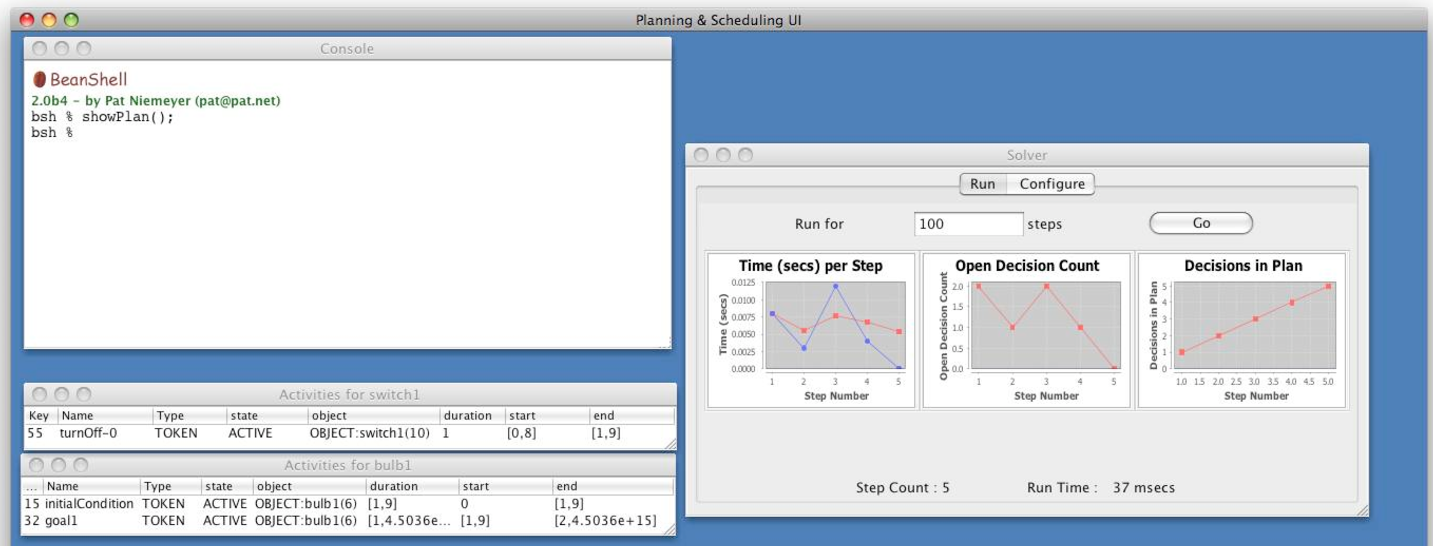
\includegraphics[width=6.5in]{./Figures/Examples-Light1.pdf}
  \end{center}
  \caption{\small UI example of the simple light-switch domain where the only action is to turn a light \emph{ON} or \emph{OFF}.}
  \label{fig:light_exp}
\end{figure*}
%--

%--
\begin{figure*}
  \begin{center}
    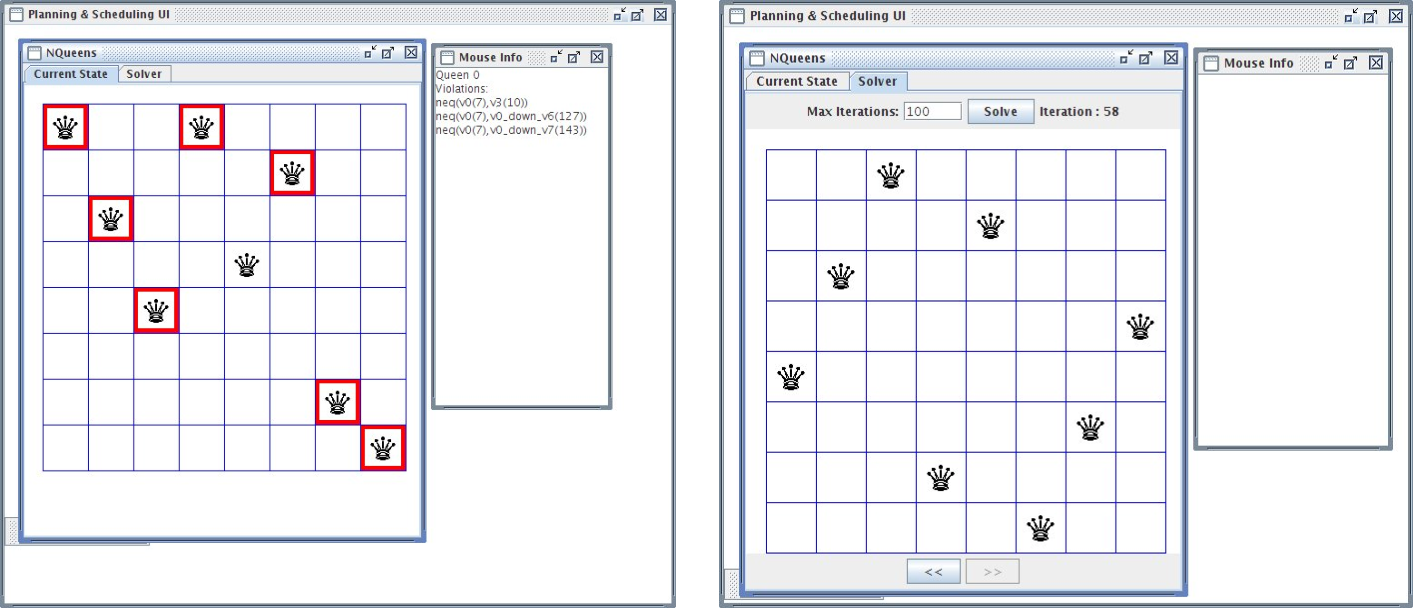
\includegraphics[width=6.5in]{./Figures/NQueens.pdf}
  \end{center}
  \caption{\small UI example of the representative Constraint Programming domain: NQueens}
  \label{fig:nqueens}
\end{figure*}
%--

%--
\begin{figure*}
  \begin{center}
    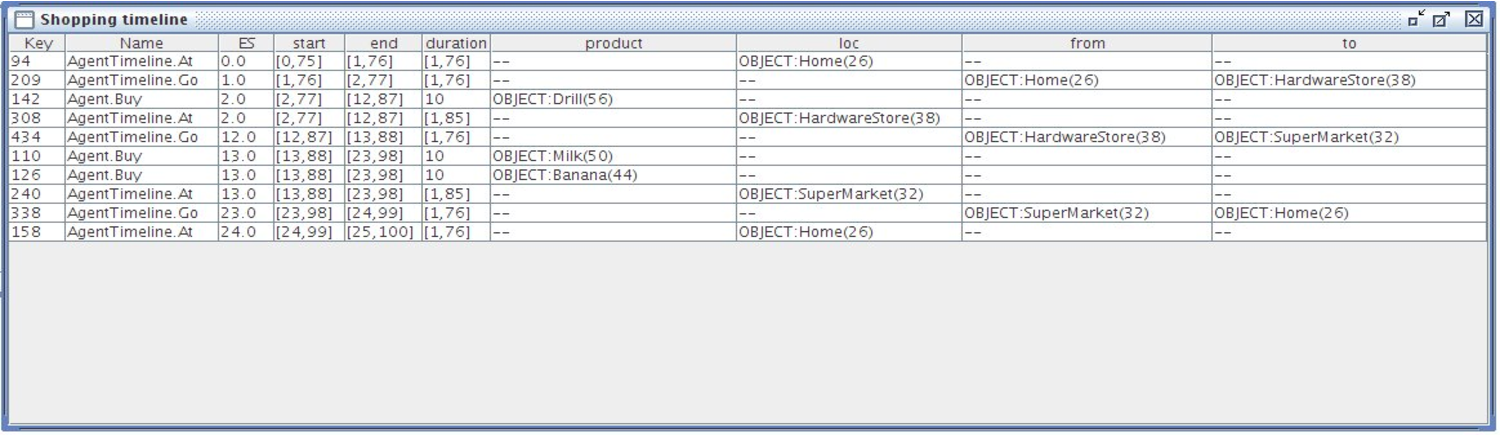
\includegraphics[width=6.5in]{./Figures/Examples-Shopping0.pdf}
  \end{center}
  \caption{\small UI example of the text-book \emph{shopping} planning example}
  \label{fig:shopping}
\end{figure*}
%--


%--
\begin{figure*}
  \begin{center}
    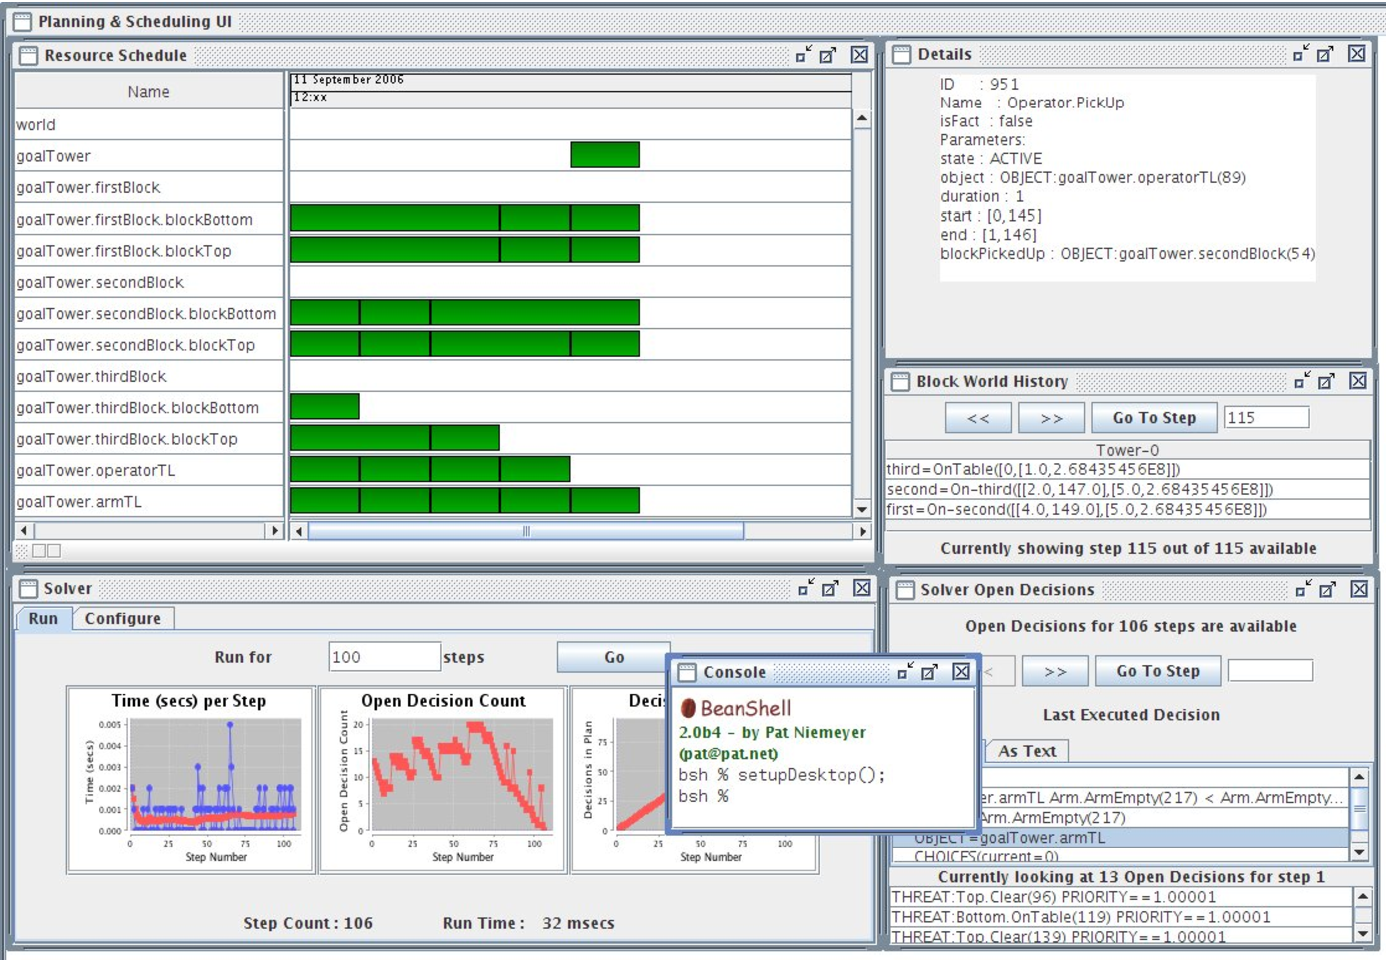
\includegraphics[width=6.5in]{./Figures/blocksworld.pdf}
  \end{center}
  \caption{\small UI example of the classical \emph{Blocksworld} planning domain.}
  \label{fig:blocksworld}
\end{figure*}
%--


%--
\begin{figure*}
  \begin{center}
    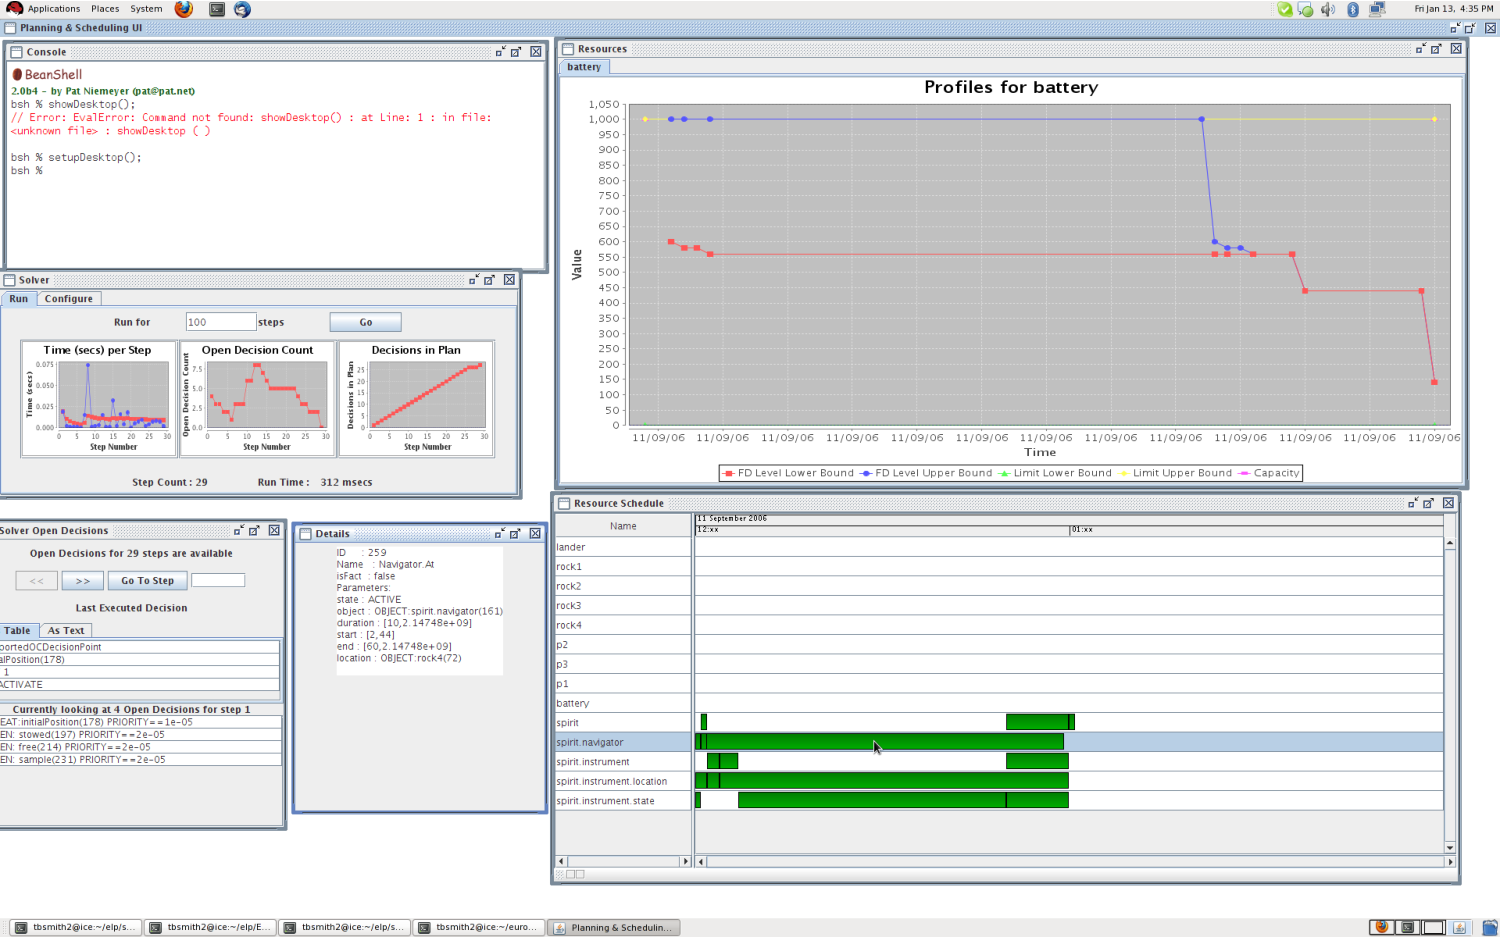
\includegraphics[width=6.5in]{./Figures/rover.pdf}
  \end{center}
  \caption{\small UI example of the \emph{Rovers} planning domain.}
  \label{fig:rover}
\end{figure*}
%--


%----------------------------
\section{\europa-related Projects}

\europa\ has been used for a variety of missions, mission-oriented research, and demonstrations, including:

\comment{JRB: I took an initial pass at this list, dropped some where europa's involvement was non material in the end. I also tried to reorganize going from production apps to prototypes. Need to make another pass}

\begin{itemize}
\item DS1: RAX �Remote Agent Experiment (original version of technology)
\item SACE Support for operation of the International Space Station's solar arrays
\item Bedrest study at Johnson Space Center
\item MER Tactical Activity Planning. \europa\ is the core planning technology behind MAPGEN, a decision support tool for generating detailed activity plans on a daily basis for the MER robotic mission to Mars.
\item Mars �03: MER �Mars Exploration Rover Science Operations
\item MSL : Support for planning and scheduling for Mars Science Laboratory Science Operations
\item Intelligent Distributed Execution Architecture (IDEA)
\item On-board Planning and Plan Execution. \europa\ was the core planning technolgoy for deliberative and reactive planning on-board a variety of mobile robots. It has been fielded in the Atacama Desert and was the cornerstone of a 2005 milestone of human-robotic collaboration for the Collaborative Decision Systems program.
\item Crew Planning Research project on Planning and Scheduling for space missions
\item ATHLETE support for foot fall planning for a lunar robot
\item STAR Advanced Spaceflight Training Systems Development
\item Mission Simulation. \europa\ was used to simulate a prospective robotic mission (LORAX) to the Antarctic for the purposes of system design evaluation.
\item Contingent Planning for ROVER operations (PiCO)
\item Personal Satellite Assistant (PSA)
\item Spoken Interface Prototype for PSA (RIALIST)
\item IS Milestone 
\item CDS Milestone
\end{itemize}

Outside of NASA, it has also beed used at MBARI to help control underwater autonomous vehicle~\cite{mcgann:2008} and at Willow Garage for autonomous robot navigation~\cite{mcgann:2009}.


%-----------------------------------
\section{Conclusion and Future Work}

In this paper, we described \europa\ with concentration on its modeling and plan analysis capabilities. The main strengths of \europa\ are: (1) expressive; (2) flexible framework; (3) strong support for integration with other applications; (4) open-source license; and (5) proven track record.

While \europa\ and its supporting tools have been going through a long period of development, we still have a long list of improvements that we want to make. The most important ones in our opinion are: significantly improve search (especially heuristic guidance) and inference capabilities, support the ANML and PDDL modeling languages, improve the visualization and debugging tools and  allow \europa\ extensions to be written in other languages. Given that \europa\ is open-source software, we welcome contributions from planning and scheduling researchers and practitioners. \\


\noindent {\bf Acknowledgements:} \europa\ is the result of many years of research, development and deployment of constraint-based planning technology.
\begin{itemize}
\item The precursor to \europa\ was HSTS, designed and developed by Nicola Muscettola. HSTS set out the initial domain description language and essentials of the planning paradigm that became the starting point for \europa.
\item Ari Jonsson led the implemenation of the first version of \europa\. Ari's team included Jeremy Frank, Paul Morris and Will Edgington, who all made valuable contributions.
\item Conor McGann led the implementation of \europa\ 2, which is a further evolution of this line of work, targeted mainly at making the technology easier to use, more efficient, easier to integrate and easier to extend. \europa\ 2's main contributors were Andrew Bachmann, Tania Bedrax-Weiss, Matthew Boyce, Patrick Daley, Will Edgington, Jeremy Frank, Michael Iatauro, Peter Jarvis, Ari Jonsson, Paul Morris, Sailesh Ramakrishnan and Will Taylor.
\item Javier Barreiro took over as the \europa\ team lead in the Fall of 2006 and has been working on it since then, improving \europa's technology and packaging. Javier's main collaborators at NASA Ames are Matthew Boyce, Minh Do, Michael Iatauro, Paul Morris, Tristan Smith and David Smith.
\end{itemize}

External contributors and collaborators include: Tatiana Kichkaylo, Mark Roberts, and Tony Pratkanis. Funding for this work has been provided by the NASA Intelligent Systems and Collaborative Decision Systems Programs.\\


{\small
\bibliography{../../../Bibliography/master}
\bibliographystyle{aaai}
}




\end{document}


%EOF
